\documentclass{base}
% Dateikodierung ist utf8
\usepackage[utf8]{inputenc}
\usepackage{url}
\usepackage[export]{adjustbox}
\usepackage{amsmath}
\usepackage{listings}
\usepackage{tikz}
\usepackage{tabularx}
\usepackage{color,colortbl}
\usepackage{ulem}
\usepackage{pdfpages}
\usepackage{ wasysym }
\usepackage{ booktabs }
\usepackage{lscape}
\usepackage{multicol}
\usepackage{longtable}
\usepackage{flexisym}
\usepackage[]{algorithm2e}

\begin{document}

\Abgabeblatt{Assignment 8}{11.6.2018}{????}{????}{Yannis Rohloff (yannis@uni-bremen.de)}{Meng Liu(lium@uni-bremen.de)}{Islam Abushanab(is\_ab@uni-bremen.de)}

\lstset{
    language=Python,
    basicstyle=\ttfamily\small,
    aboveskip={1.0\baselineskip},
    belowskip={1.0\baselineskip},
    columns=fixed,
    extendedchars=true,
    breaklines=true,
    tabsize=4,
    prebreak=\raisebox{0ex}[0ex][0ex]{\ensuremath{\hookleftarrow}},
    frame=lines,
    showtabs=false,
    showspaces=false,
    showstringspaces=false,
    keywordstyle=\color[rgb]{0.627,0.126,0.941},
    commentstyle=\color[rgb]{0.133,0.545,0.133},
    stringstyle=\color[rgb]{01,0,0},
    numbers=left,
    numberstyle=\small,
    stepnumber=1,
    numbersep=10pt,
    captionpos=t,
    escapeinside={\%*}{*)}
}


\section*{Mixed-integer linear programming in practice}

\lstinputlisting{alloy.lp}

We added 4 variables to the original solution. $lim_A$ to $lim_D$ describe if, for any of the four recycled materials, the percantage is below 0.2.
If it is above, the value needs to be higher that zero. If it is higher than 0 this adds an additional 20 dollars to the total cost.
Technically for any material the solver could set $lim_A$ to two and would therefore add 40 dollars to the total price, but since $lim_A=1$ always suffices that would never be the case.

\clearpage
\section*{Non-convexity in LP and ILP solving}
A non convex solution space cannot be expressed by linear programming.
If it could be expressed the simplex algorithm would not work for this instance.

The following image illustrates two possible paths the simplex algorithm would walk from the starting point, whereas only the red path leads to the correct optimum.
Since the simplex algorithm can calculate the optimum for any LP instance our instance cannot be a linear programming instance.

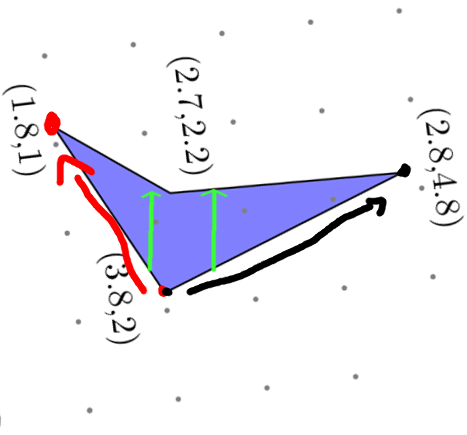
\includegraphics[scale=0.5]{rotated.png}

We still tried to model it with linear programming by encoding every edge with the formula given by the task.
This yields the code in \verb|area.py|.
But logically the solution space is constrained by a line and not by a line segment.

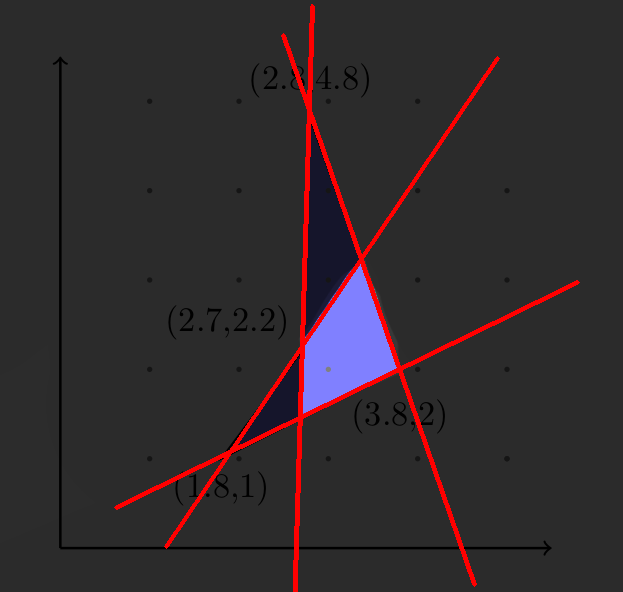
\includegraphics[scale=0.5]{solution_space.png}


The trick could still be to use integer linear programming. Now we can add an additional helper variable that helps us to make a hard decision: a boolean decision if if an edge should be taken into account for a given point or not.
In this example we can add a condition for both edges on th non-convex part. If $x>=2.7$ we want to only use the upper edge. If $x<=2.7$ we want to ignore the upper edge and only constrain.

The code for both solutions:
\lstinputlisting{area.py}

\clearpage
\section*{Challenge \& Bonus Problem: Cleaning up a Mess}
We already thought about this but did not yet come up with a solution.

\end{document}
